\documentclass{article}
\usepackage{../../Self_Style}

\title{Phys 20AL Lab Report Week 4: Mass and Spring}
\author{Zih-Yu Hsieh}
\date{\today}

\begin{document}
\maketitle

\tableofcontents

\section{Introduction}
For a simple/ideal spring, the  magnitude of the force it applies when being stretched is observed to be proportional to the stretched distance , and with direction opposite from the direction it is being pulled. Which, let proportionality constant be denoted as $k>0$, the associated differential equation is given as $F = m \ddot x = -k x$, which represents an equation for a Simple Harmonic Oscillator (SHO). As a result, the idealized spring as an SHO would have its period provided as $\tau=2\pi\sqrt{\frac{m}{k}}$ after solving the differential equation.

\hfill

The experiment is to measure the spring constant of a spring provided in the lab. In addition, it'll also be focusing on the static relation between the mass and the spring stretch of a spring, together with how variation of mass and maximum amplitude would affect the time period of a spring's dynamic motion.

\newpage

\section{Experimental Setup}
Here there are three different sets of experiments: Two of the experiments - one measures the static scenario, the other measures the dynamic of the spring - record data manually, whil the third one (which is also measuring the dynamic of a spring) has an associated electronic detector. The details are described as below.

\subsection{Experiments Recording data Manually}
For this setup, there are two experiments involved: Collecting data of the spring's stretch under static scenario, and collecting data of the object's period under dynamic scenario.

The equipments include: Stand, two clamps, spring (that can endure long enough stretch without explicit deformation, typically a stretch of near $1$ m), meter stick, a hook of $50$ g, timer, mass scale, and masses of one $50$ g, two $100$ g, and one $200$ g.

The following is the steps for setup:
\begin{itemize}
    \item[1.] Setup the stand at the edge of the table.
    \item[2.] Fix one of the clamp on the top of the stand, and clamp one end of the spring onto it.
    \item[3.] Fix the other clamp near the middle of the stand, and clamp the meter stick vertically onto it.
\end{itemize}
\begin{figure}[h!]
    \centering
    \begin{subfigure}[t]{0.4\textwidth}
        \centering
        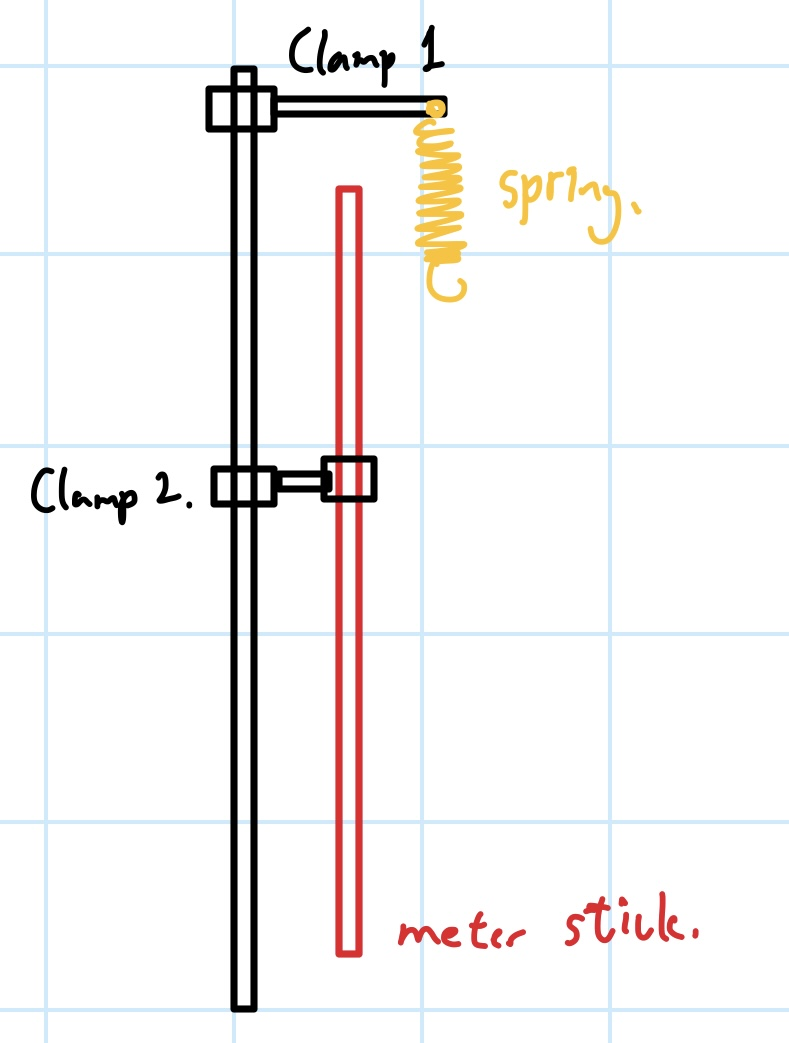
\includegraphics[width=40mm]{setup_sketch_manual.jpg}
        \caption{Sketch of the Setup with Manual Data Recording}
        \label{fig:sketch_setup_manual}
    \end{subfigure}%
    \hfil 
    \begin{subfigure}[t]{0.25\textwidth}
        \centering
        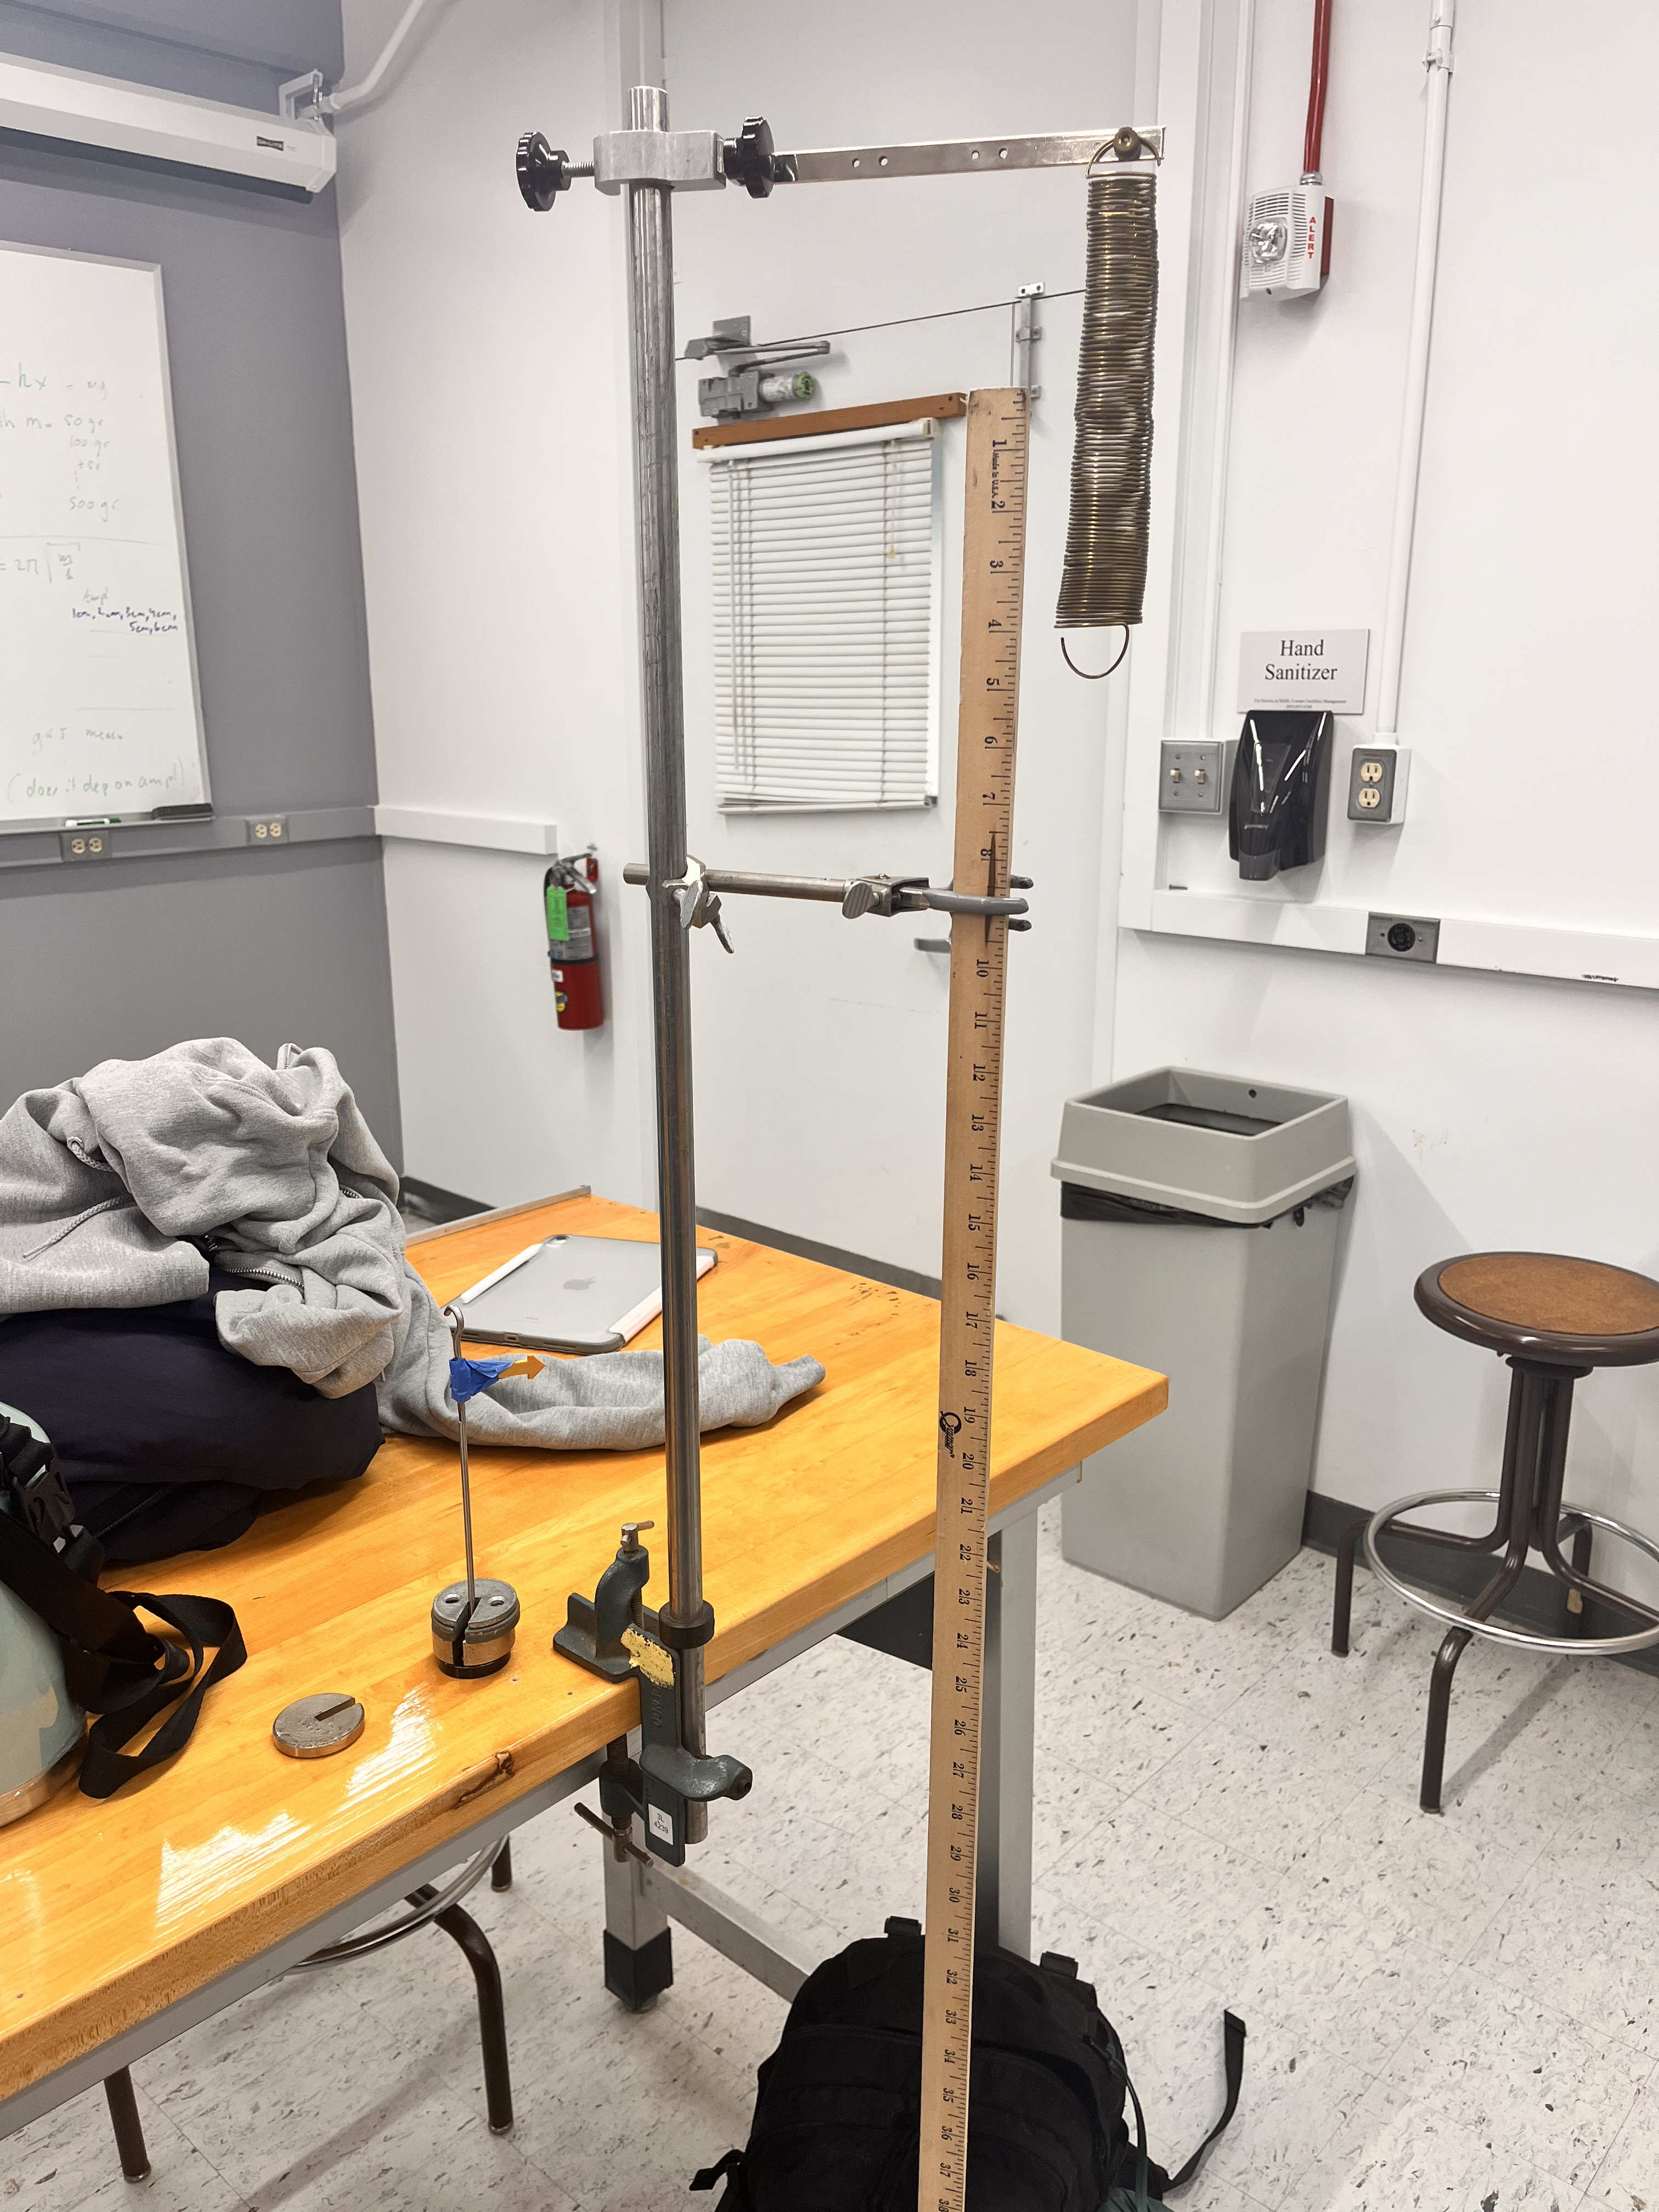
\includegraphics[width=\linewidth]{setup_manual.png}
        \caption{Photo of the Equipment Setup}
        \label{fig:setup_manual}
    \end{subfigure}
\end{figure}

\subsection{Experiment Recording data with Detector}
For this setup, there is only one experiment, which is using the electronic detector to record the dynamic motion of the simple harmonic oscillator.

The equipments are nearly the same as in \textbf{Section 2.1}, except now it requires one more clamp, an electronic detector, and a computer.

The setup steps mostly follow from the one in \textbf{Section 2.1}, just in addition one needs to use the extra clamp to fix the detector on the stand, and plugin the detector to the computer for data recording.
\begin{figure}[h!]
    \centering
    \begin{subfigure}[t]{0.4\textwidth}
        \centering
        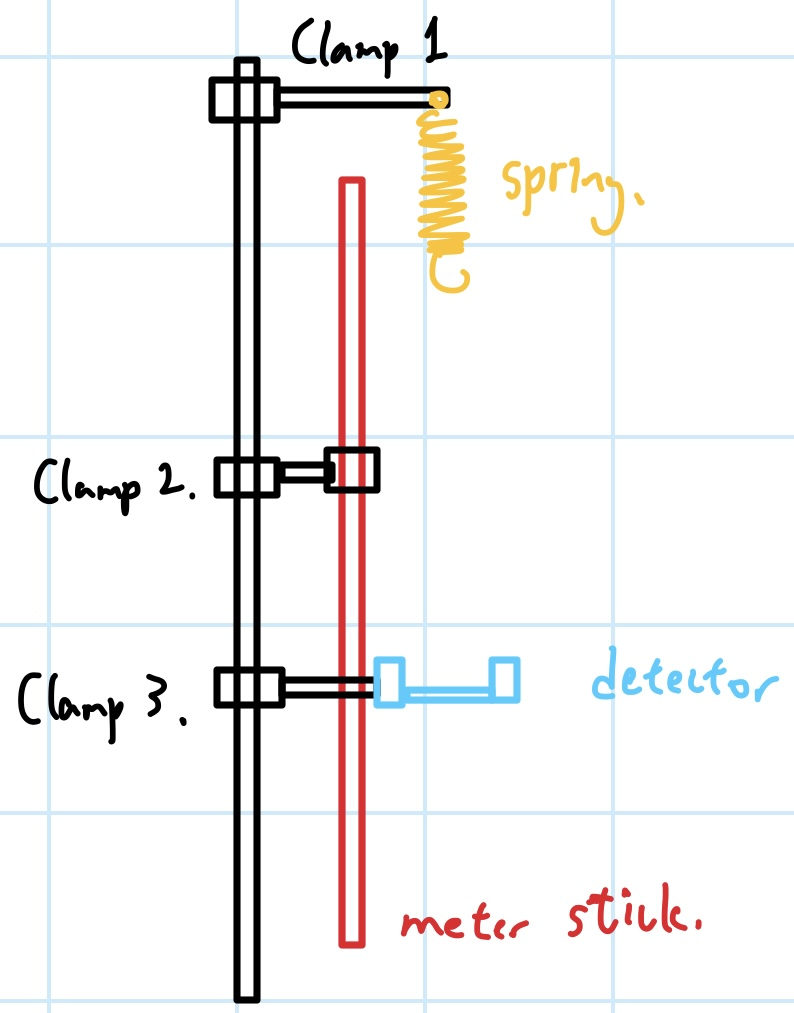
\includegraphics[width=40mm]{setup_sketch_detector.jpg}
        \caption{Sketch of the Setup with Manual Data Recording}
        \label{fig:setup_sketch_detector}
    \end{subfigure}%
    \hfil 
    \begin{subfigure}[t]{0.25\textwidth}
        \centering
        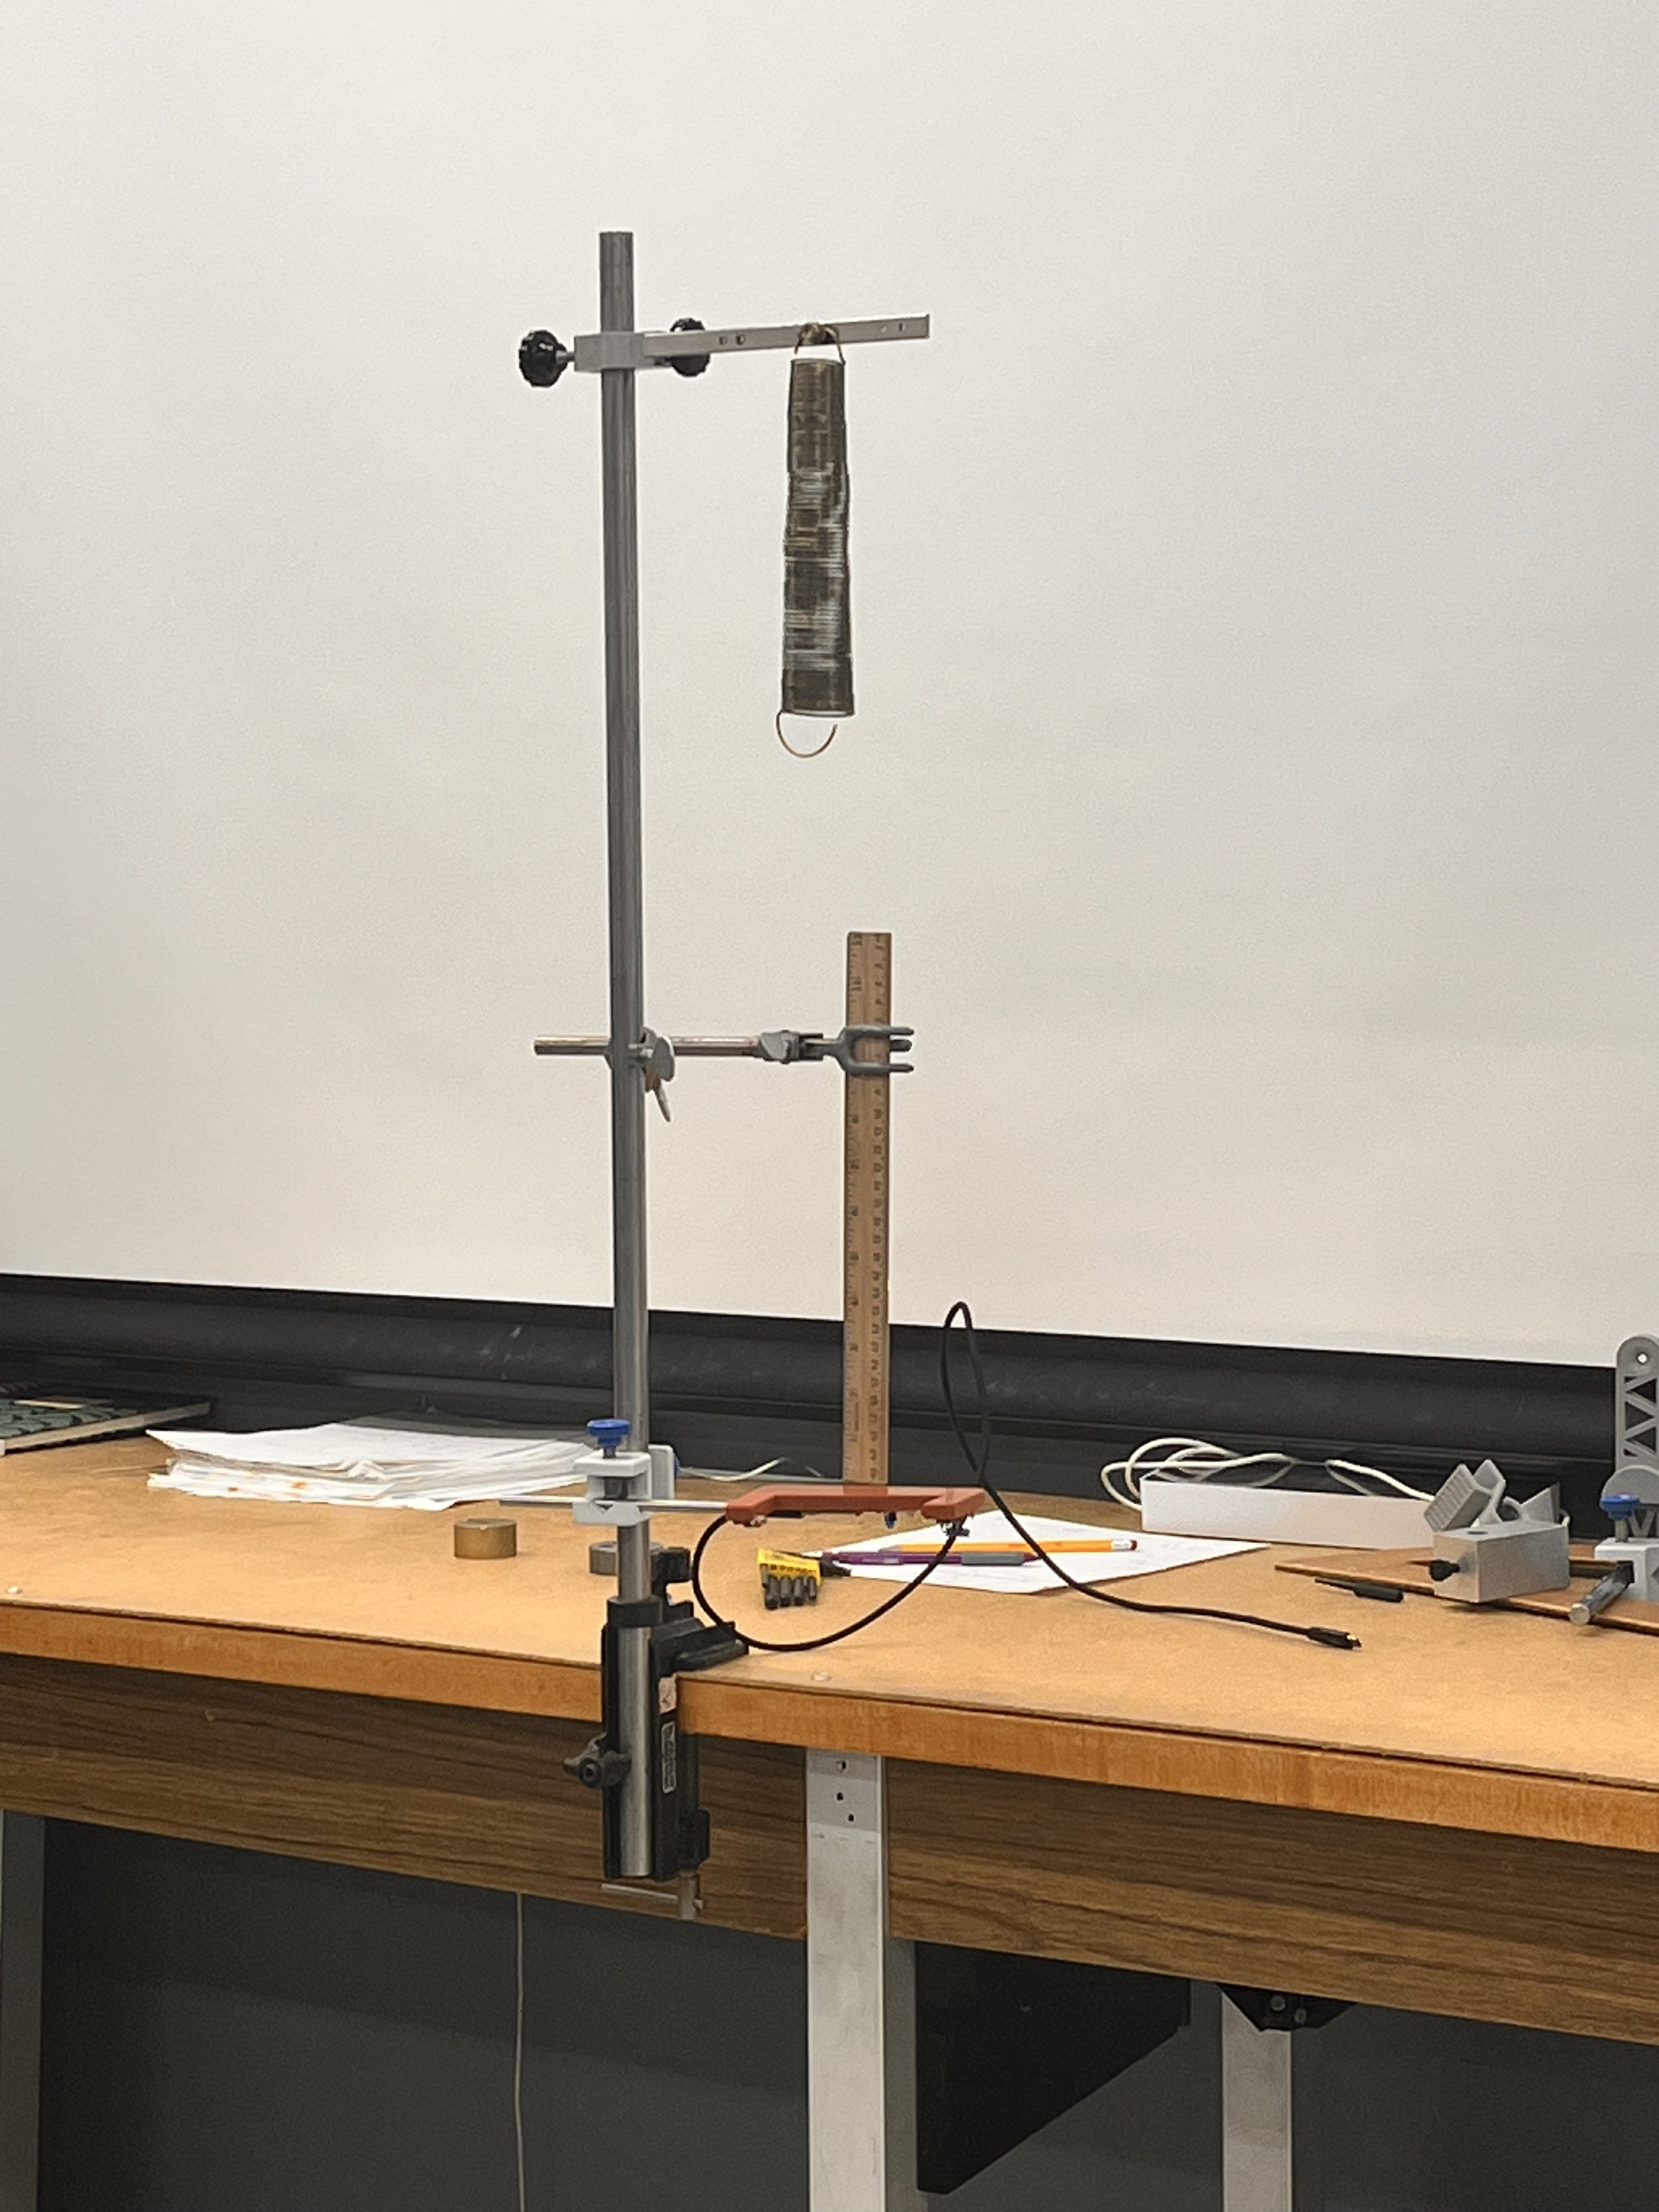
\includegraphics[width=\linewidth]{setup_detector.png}
        \caption{Photo of the Equipment Setup}
        \label{fig:setup_detector}
    \end{subfigure}
\end{figure}


\section{Methods of Measurement and Procedure}

\section{Experimental Data and Tables}

\section{Data Analysis}

\section{Error Analysis}

\section{Conclusion (Includes Experimental Improvement)}

\end{document}